
\documentclass[a4, 10pt,dvipdfmx]{jsarticle}

%\usepackage[chukan]{sotsuron}
%\usepackage[dvips]{graphicx}

%\setlength{\topmargin}{-13truemm}
%\setlength{\headheight}{0mm}
%\setlength{\headsep}{0mm}
%\setlength{\textheight}{45\baselineskip}
%\setlength{\textheight}{26cm}
%\addtolength{\textheight}{\topskip}
%\addtolength{\textwidth}{5cm}
%\addtolength{\oddsidemargin}{-2.5cm}

\usepackage[dvipdfmx]{graphicx}
\def\pgfsysdriver{pgfsys-dvipdfmx.def}
\usepackage{threeparttable}
\usepackage{tikz}
%\usepackage[chukan, nobroaderlayout]{sotsuron}
\usepackage[chukan]{sotsuron}
\usepackage{ascmac}
\usepackage{bm}
\usepackage{amsmath}
\usepackage{fancybox}
\usepackage{url}

\begin{document}

\makecover

\pagenumbering{roman}

\tableofcontents

\newpage

\pagenumbering{arabic}

\section*{概要} 

% 実世界では多くの交渉が行われており、競争的状況において自分の利益を最大化することを目指している。このとき、交渉相手の利益など交渉成立の要件も考慮した上で、自分の利益を最大化できる交渉を相手に提示し、自分にとって不利な交渉は受けないようにする必要がある。利益を最大化する交渉を探る手法の1つとして、実世界をモデル化した知能ゲームをコンピュータに解かせる方法がある。知能ゲームの研究は、情報システムによる支援などの実世界において実用的価値を持ちうるため、これを交渉にも適用する。
% 本研究では、これを現実社会に似たモデルである、「カタンの開拓者」というマルチエージェント、不完全情報、非決定的なゲームを用いて評価検証を行う。このモデルにおいて、最適な交渉案を評価する関数(評価関数)を提示することで、現実世界での応用が期待できる。交渉では、互いの利益計算を行なう必要があり、モンテカルロ木探索が先読みの有効な手段だという仮説のもと、これを用いて互いの利益計算を行い、簡単なルールベースに基づく交渉を行うプレイヤーと比較することでその性能を評価する。また、得られた利益に基づいて交渉の評価関数をいくつか提示し、その中から自らの利益を最大化する評価関数を提案し、交渉における重要な要素の検証を行なった。


実世界では多くの交渉が行われており、競争的状況において自分の利益を最大化することを目指している。交渉の研究の多くは、定性的な研究であり、定量的な交渉の研究は未だ発展途上である。その理由として、先読みによって得られる利益を数値化し、どのような交渉を提示するかの指標となる評価関数を用意する難しさにある。本研究では、先読みによる利益計算に、近年成功をおさめているモンテカルロ法を適用することを提案し、また、指標となる様々な評価関数を提示する。モンテカルロ法が利益計算において有効な手段であるかどうかを検証し、また、評価関数の比較実験を行なう事で交渉において重要となる要素を検証することを目的とする。実験結果より、モンテカルロ法は利益計算に有効であるとは言えなかった。しかし、交渉の評価関数を生成する上で、「提案成功率」「受諾率」「自分の利益」のみならず、「相手の損益」を考慮した評価関数を生成する必要があることが分かった。


 % 。また、交渉の内容を自分の利益を最大化し相手の利益を最小化する場合、相手の利益を最大化し自分の利益を最大化する場合、お互い利益を分け合う場合の3つのパターンに分け、他のプレイヤーが交渉に応じる分布を調べる。ゲームでの研究が、実社会での交渉についての情報システムによる支援などの実用的価値を持ちうる

\section{はじめに}

\subsection{背景}
% ~\cite{}

現実社会では、多くの場面で関係者間に利害関係があり、その解決のために様々な交渉が行われている。
交渉の研究は社会科学的な研究が多く、戦略やノウハウといった定性的な交渉術~\cite{fisher2011,lewicki2001essentials,岡紀子2002視点}としての研究が中心となっている。
そのため、交渉において定量的な交渉術の研究は未だ発展途上であり~\cite{安村禎明2002モノポリーゲームにおける交渉エージェント}、決定的な解は見つかっていない。

決定的な解が見つかっていない理由として、自分が最も有利となる交渉案を定量的に選択する難しさにある。
ひとつ目は、交渉によって得られる利益を数値化することの難しさである。正確に利益を数値化するには、現在の状態を考えるだけでは不十分であり、不確実な将来に得られる利益を含めるのは困難である。
ふたつ目は、相手が交渉を受ける可能性を、定量的に評価する難しさである。もし、正確な先読みによって利益計算を行い、自分にとって最も利益の高い交渉を相手に提示したとしても、相手が受諾しなければ、自分は利益を得ることができない。そのため、相手が交渉をうける可能性を考慮し、自分の利益の期待値を最大にする交渉案を生成する評価関数が必要である。

また、交渉を行う人工知能を、実世界の条件のままコンピュータ上に設計する事は困難である。なぜなら、実世界の問題では、とりうる状態が無数に存在し、各々から遷移しうる先の状態がまた無数にあり、遷移が可能になる条件も複雑である。よって、実世界をモデル化するために、実世界の特徴となる要素を抽出し設計する必要がある。

実世界の要素を抽出した知能ゲームをコンピュータ上に設計しプレイさせて、実世界に応用する研究 ~\cite{川越敏司2010行動ゲーム理論入門}が以前から行われている。
一般に実世界をモデル化したゲームの要素を、多人数ゲームであるか、確率的な要素を含むか、ある状態の情報がわかっているか、という軸でわけることが多い。
多人数でプレイしたり、不確定あるいは不完全な情報しか得られないゲームが、最も実世界近いゲームである。しかし、多人数ゲームはプレイヤー同士の協力関係を持つと戦略を変える必要があり、また、不確定不完全情報ゲームは、偶発的なイベントで状況が変動するため探索空間が大きくなるため純粋な先読みが難しい。本研究では、この知能ゲームとして「カタンの開拓者」(以下カタン)というゲームを用いて評価検証を行なった。

\subsection{目的}

自らの利益の期待値を最大にする交渉を定量的に検証するために、利益を数値化し、評価関数を用いて交渉を選択する必要があった。
本研究では、先読みによる利益計算に、ランダム試行に基づくモンテカルロ法を適用し、その有効性を検証することを目的とする。モンテカルロ法は人工知能の分野で多くの成功をおさめているため、利益計算に応用できると期待される。また、交渉の選択を行なう評価関数として、様々な評価関数の比較実験を行なう事で交渉において重要となる要素を検証することを目的とする。

\subsection{本研究の貢献}

利益計算において、簡単なルールベースとモンテカルロ法の一致率を検証することで、モンテカルロ法による利益計算の問題点がわかった。
また、交渉案を選択する評価関数を生成する時に、悪い交渉案を混ぜることが有意な結果を残したことから、「相手の損益」を考慮した評価関数が有効であると考えられる。
本研究によって得られたゲームモデルにおける交渉案選択手法は、他の実世界に近いゲームモデルで応用することが可能である。

\subsection{本稿の構成}

本稿は、第2章で関連研究の紹介、第3章で提案手法を説明し、第4章で実験方法、第5章で評価を示し、最後に第6章でまとめと今後の課題ついて述べる.


\section{関連研究}

本章では、多人数ゲームシステムの説明を2.1節で行い、本研究のメインテーマである交渉に関する説明を2.2節で行う。

次に2.3節、2.4節において、交渉の評価値を計算するUCTアルゴリズムについて説明する。

\subsection{多人数ゲーム}
自ら考え行動し、人間に変わって複雑な作業などを代行するものを「エージェント」と呼ぶ。そのようなエージェントが多数共存する環境を、多人数ゲームと呼び、複数のエージェントが協調して解決しようとするシステムがマルチエージェントシステムである。社会にはいくつもの要素が絡み合う複雑な事象が溢れており、個々のエージェントの動きだけでは想定できないようなマクロな現象をボトムアップ的に解析することが可能となる。

\subsection{交渉}
2.2.1節で一般的に行われている交渉のパターンを紹介し、2.2.2節で交渉の手順について述べる。最後に2.2.3節で交渉のアルゴリズムを紹介する。

\subsubsection{協力型交渉と競争型交渉}
交渉には大きく協力型交渉と競争型交渉がある~\cite{anguix2013complex}。一般に、競争型交渉は協力型交渉に比べて難しい。なぜなら、協力型交渉はお互いの情報が開示されている場合がほとんどで、お互いの利益を最大化するだけでよい。そのため、交渉は成立しやすい。一方で、競争型交渉は多くの場合お互いの情報が開示されておらず、また、各々のエージェントが自分の利益のみ最大化することを考えるため、交渉は決裂することが多い。そのため、妥協点をいかにうまく設定するかが、現実世界でも大きな課題である。

また、一般的に競争型交渉は価格交渉のようにゼロサムゲームを想定し、最初の交換提案をどの程度に、それぞれがどのように譲歩するかを決定する。しかし、交渉によっては交換する資源の組み合わせを変更する事で、双方の利益をふやすことができる場合があり、単なるゼロサムゲームでないゲームもある。このような交渉形態は、利益交換型交渉~\cite{開発2009kobe}と呼ばれ、ゼロサムゲームである分配型交渉よりも良い交渉形態である。この交渉を扱うことができることも、カタンで交渉の研究を行なう利点となる。

\subsubsection{交渉の手順}
交渉において各々のプレイヤーは以下のような手順で交渉の成立を目指す~\cite{安村禎明2002モノポリーゲームにおける交渉エージェント}。
\subsubsection*{候補の列挙}
基本的に、交渉を行うときは、他のプレイヤー全てと交渉することが可能である。全てのプレイヤーに対して、1対1、1対多、多対多の交渉内容を列挙する必要がある。

\subsubsection*{候補の選択}
列挙した候補の中から、交渉を選択する基準(ゲームの場合は、評価関数)に基づいて評価し選択する必要がある。それぞれの候補に対して、交渉を行った事よって、お互いの利益の増加がおこりえるが、相手と自分の利益が同程度上昇しない限りは基本的に交渉は成立しない。
それぞれの交渉に対して「正確な利益を計算し、利益に基づいた良い選択基準」を作る事が交渉を成立させる重要な要因である。
また、交渉相手が消極的なエージェントであった場合、自分にとって少し有利な条件を選択する評価関数に変更することができる。

\subsubsection*{交渉の切り出し}
評価関数に基づいて選択した候補の中から、そのうち上位のいくつかを選択して提案する。これは、現実世界において同じ相手に対し、全ての交渉案を提案することはほとんどないためである。交渉内容をある程度しぼって提案する必要がある。これらが実際に相手に提案する交渉案となる。また、相手に提示する交渉案の順番によって、交渉の成功確率が変化することがある。

\subsubsection*{交渉の成立}
相手が自分の提案した交渉内容を受諾した場合、交渉成立となる。また、提示した交渉案が受諾される事なく、相手によって新たな条件で提案される場合は、相手が提案してきた交渉内容が自らの評価関数に基づいた交渉順位のどこに位置するかをみることで、お互いが受け入れるラインを再度提案する。
一定の提案回数で交渉が成立しない場合は、交渉決裂となる。

\subsubsection{交渉に関するアルゴリズム}
交渉を行なう場合、お互いの評価関数が異なっているため、自分の評価関数であれば受諾する交渉でも、相手の評価関数では受諾を選ばず、結果交渉が成立しないということがある。
交渉が決裂すると、実際に得られるはずだった利益を得られなくなることにより、機会損失を招いてしまう。そのため、交渉においてはお互いの妥協点をみつける必要がある。

妥協点を見つける方法として、相手のモデル化~\cite{baarslag2012evaluating}がある。例えば、IAMhaggler2011は序盤の交渉でガウス過程的~\cite{rasmussen2006gaussian}にモデル化を行なう事で、相手の利益を予測することができる。これを適用したIAMhaggler2011~\cite{williams2013iamhaggler2011}とい人工知能は、ANAC(Automated Negotiating Agents Competition、以下ANAC)にて優秀な結果を残している。IAMhaggler2011は相手の利益を予測した後、自分の利益を最大化する交渉案が最もよい結果を残している。

また、交渉案を選択する評価関数の譲歩率を測定する方法\cite{baarslag2012evaluating}がある。譲歩率は機会損失をさける指標となる。
ANACにて優秀とされる結果を残した人工知能~\cite{baarslag2012evaluating}は、一定の譲歩を行なっていることから、自分の利益のみを考える評価関数が優位な戦略でないと考えられる。



%そこで、交渉の成功率をあげる方法として、相手のモデル化がある。相手のモデル化を行なう複数のプレイヤーの中で対戦実験を行い、相手プレイヤーは必ず交渉を成立することを優先すると仮定して、ほとんど譲歩しない交渉に消極的なプレイヤーが最も良い結果を出した。本研究でも相手の交渉をなるべく消極的なプレイヤーを用意することで、交渉の評価基準の性能を評価する。

% \subsection{交渉の評価}
% 交渉内容を評価する論文をまだ探していない。



% \subsection{非決定的な問題}
% 決定的アルゴリズムは、入力を与えられたとき、常に同じ経路で計算を行い、常に同じ結果を返すため動作が予測可能なものをいう。一方では非決定的アルゴリズムは入力が与えられたときに常に同じ結果を返すわけではない。例えばサイコロを振ると行った確率的なモデルがこれにあたる。非決定的アルゴリズムは、常に同じ結果を返すわけではないので、解を求めるためにしらみつぶしに探索を行う必要がでてくる。そのため、探索空間が決定的アルゴリズムよりも急激に大きくなるため、難しいとされている。

% \subsection{不完全情報}
% 完全情報とは、エージェントが意思決定を行う全ての点において、これまでにとられた行動や実現した状態に関する情報が全て与えられていることをいう。一方で不完全情報はエージェントが意思決定を行う全ての点において、これまでとられた行動や状態が全て与えられていない状態が存在することをいう。一般に、不完全情報ゲームは完全情報ゲームに比べ、確率的や統計的な予測が入るため強さの比較が難しいという問題点が挙げれる。

\subsection{UCTアルゴリズム}

まずモンテカルロ法について説明する。モンテカルロ法は、状態の評価が難しい問題において有効とされる手法である。

モンテカルロ法は、ある局面から終局までランダムに行われる試行に基づき統計的に評価する。これはプレイアウトと呼ばれ、プレイアウトを繰り返す事で、ある局面の勝率を計算することができる。最も単純なモンテカルロ法は、ある局面の合法手を行ったところからプレイアウトを開始して、毎ターン勝率を計算し、最も勝率の高いものを選択するものである。

\begin{figure}[b]
    \begin{center}
      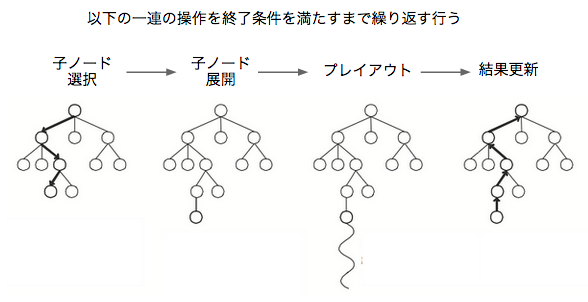
\includegraphics[width=120mm]{img/monte_carlo.png}
    \end{center}
    \caption{モンテカルロ木探索~\cite{kocsis2006bandit}}
    \label{monte_carlo}
\end{figure}

しかしながら、有限な時間内に正確な勝率評価を行う場合、明らかに有望と思われない手に対して、有望な手と同様の試行回数を行うことは無益である。よって、これを解消するため有望な手にバイアスをかけて試行回数を配分する必要がある。これがUCBアルゴリズム(Upper Confidence Bound、以下UCB)である。 


バイアスをかけて子ノードを選択する場合、まず未探索の子ノードを優先的に選択する。子ノードが全て探索済みの場合は、以下の式が最大となる子ノードを探索することで、探索回数が少なく、高い報酬を得る可能性のある手に対して第2項が大きくなるため探索されやすいというアルゴリズムである。探索回数が多くなると、第1項の平均報酬の高い手が基本的に選択される。
\begin{equation}
  UCB(j)=\overline{X_j} + C\sqrt{\mathstrut \frac{\ln{n}}{n_j}}
\end{equation}
但し、$\overline{X_j}$ は現在の状態までの試行で算出した平均勝率、$C$ は調整パラメータ、$n$ は全ての合法手の試行回数の合計、$n_j$ は合法手 $j$ の試行回数とする。

選択したノードをプレイアウトした後は、その結果を報酬として探索経路上のノードを更新する。

以上の「子ノードの選択」「子ノードの展開」「プレイアウト」「結果の更新」を終了条件 (時間や探索回数など)となるまで繰り返し、平均報酬の最も高い子ノードを次のアクションとする。
本研究では、モンテカルロ木探索にUCB値を用いた探索であるUCTアルゴリズム~\cite{kocsis2006bandit,auer2002finite}によって得られた子ノードの平均報酬の結果を用いて、交渉の評価関数を生成することとなる。

また、モンテカルロ法のアルゴリズムであるモンテカルロ木探索(Monte Carlo Tree Search、以下MCTS)をカタンのAIであるJSettlersに適用し、成功をおさめている~\cite{branca2007using}。
JSettlersのプレイヤーに対して、JSettlersをベースとしたMCTSの0回シミュレート、1,000回シミュレートおよび10,000回シミュレートを行った。
1人のSmartSettlersプレイヤー、他の3人JSettlersを用いたプレイヤーに対し、25\%、27\%、49\%の勝率を残し~\cite{szita2010monte}、カタンにおけるMCTSがランダムプレイヤーよりは強いことを示している。

\subsection{多人数ゲームにおけるUCTアルゴリズム}

多人数のゲームでは2人のゲームに比べてUCTよりも評価関数による局面評価が難しい。~\cite{sturtevant2008analysis}

\begin{figure}[t]
    \begin{center}
      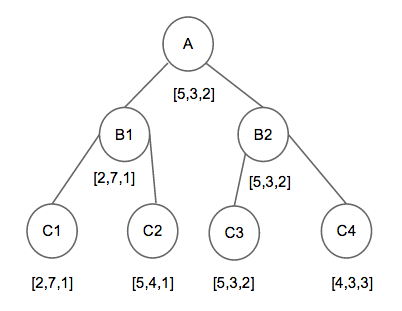
\includegraphics[width=80mm]{img/multi_agent_tree.png}
    \end{center}
    \caption{多人数ゲームの評価値例}
    \label{multi_agent_tree}
\end{figure}

図2のように、各ノードが自分のノードの値を最大とする手を選んでいるものとする。ここで、敵となるプレイヤーが2人いるため、敵がどちらを選択すべきか判断するためには2人の戦略モデルを知る必要がある。しかし、一般に適切な戦略モデルを作成することは難しい。
一方で、これにUCTアルゴリズムを適用するとノードB2ではプレイヤーBが返す報酬は同じであるため、UCB値による手の選択は探索回数によって決定される。
結果、両方の子ノードは同じ回数探索が行われ、親のノード2の評価値は2つのノードの平均値をとることになる。これにより、他のプレイヤーに対しての混合戦略~\cite{nash1951non}を得る事ができる。

以上より、UCTアルゴリズムを多人数ゲームで使用すると、シミュレーションに基づいた探索が行われるため、相手よって戦略が異なる場合がでてくる。そのため、これらの戦略をうまく組み合わせた戦略(混合戦略)を考える必要性がある。実際、UCTアルゴリズムは評価関数を用いたMaximum探索よりも高い性能を発揮している。


\section{提案手法}

本研究では、現実世界のモデルに近い、不完全情報ゲーム、非決定的、多人数ゲームという要素をもつことから、カタンの開拓者を用いて検証する。
交渉を行なうときに以下の手順を踏むものとする。
\begin{itemize}
 \item 全てのプレイヤーに対して可能な交渉案のリストアップ
 \item 各交渉案の利益の見積もり
 \item 評価関数による各交渉案の期待値計算
 \item 交渉案の提示
\end{itemize}
自分のターンにおいて、初めに、全てのプレイヤーに対して可能な交渉案を求める。次に、これらの交渉案に対して、ルールベースもしくはUCTアルゴリズムを用いて、利益の見積もりを行なう。
そして、見積もりの結果を用いて、提案した評価関数に基づき、交渉による各交渉案の期待値を計算する。最も自分の利益の高い交渉案を提示せずに、評価関数を用いて期待値を計算する必要があるのは、相手が受諾するかどうかを考慮する必要があるからである。最後に、最も期待値の高い交渉案を提示する。交渉は自分のターンに1回限りとする。

以下、本章では、まず交渉の利益計算方法について3.1節で説明し、3.2節で交渉を選ぶ評価関数を説明する。

\subsection{交渉の利益見積り}

交渉を提案する上で自分と相手の利益を計算する必要がある。利益を以下のように計算するものとする。

利益計算において、先読み手法であるUCTアルゴリズムを用いることが本研究の提案の1つである。
UCTアルゴリズムによるプレイアウトによって、各プレイヤーの勝率を計算することができる。交渉による損得は最終的に自分の勝率に直結することから、UCTアルゴリズムの先読みによって予め得た勝率により利益計算を行なうことができると考えられる。よって、UCTアルゴリズムの先読みによって得た勝率を、利益計算に用いる事にする。  
まず、交渉を行わなかった場合の勝率を$x$、交渉を行って成功した場合の勝率を$x_{trade}$とする。

\begin{equation}
  R = x_{trade} - x
\end{equation}
「利益($R$)=交渉をおこなった場合と行わなかった場合とを比べて、自分の勝率が何ポイント上昇するか」

「それぞれの交渉を行って成功した場合」と「交渉を行わなかった場合」について勝率の違いを求める。
\begin{itemize}
 \item 交渉を行わなか
    \begin{itemize}
      \item プレイアウトした時の自分プレイヤーAの勝率 $W_a$
      \item プレイアウトした時の相手プレイヤーBの勝率$W_b$
     \end{itemize}
 \item 交渉を行なって成功した
    \begin{itemize}
      \item プレイアウトした時の自分プレイヤーAの勝率 $Wt_a$
      \item プレイアウトした時の相手プレイヤーBの勝率 $Wt_b$
     \end{itemize}
\end{itemize}
すなわち各々のプレイヤーの利益は以下のようになる。
\begin{eqnarray}
  R_{a}=Wt_a - W_a
\end{eqnarray}
\begin{eqnarray}
  R_{b}=Wt_b - W_b
\end{eqnarray}


\subsection{交渉を選ぶ評価関数}
相手のプレイヤーが自分の提案した交渉を必ず応じてくれることはなく、自分の利益を最大化しつつ、相手が受諾しやすい交渉案を提示する必要がある。
プレイヤー間では競争的交渉が行われるため、その中で妥協点をみつけ出す必要がでてくる。すなわち、妥協的交渉を行う方法を考える必要がある。
それぞれの交渉に関して評価値を設定する事により、評価値が最も高くなる交渉を提案することにする。ただし、全ての交渉案に対し、交渉をしない方が評価値が高い場合は交渉を行なわないものとする。  
\begin{equation}
  v_{best} =  \max_{i}f(s_{i}) ( s = 1, 2, \cdots, N )
\end{equation}
「最大の評価値($v_{best}$)=最も高い評価値の交渉案」
「評価関数($f(s)$)=ある交渉案に対して評価値を求める関数」
「交渉案($s$)=提案することのできる交渉案」

本研究では、前節で得られた利益計算の結果を用いて、交渉の成功率を考慮した評価関数により交渉を提示する。
自分の利益を最大化しつつ、交渉の成功率をあげる必要がある。交渉の成功率は「相手が得られる利益」に影響を受けるものだと仮定する。
よって、良い交渉案を選ぶ評価関数として、以下の5つの評価方法を提案することにする。
まず、自分の利益のみしか考えない「自己中心的交渉」を行なうプレイヤーをベースラインとして扱う。次に、交渉の成功率よりも相手の利益を優先にした「利益優先交渉」と交渉の成功率を優先した「受諾優先交渉」を提示する。また、お互いの利益をバランスよく配分することで、自分の利益と交渉の成功率を調整する手法として「和交渉」「積交渉」を提示する。

\subsubsection*{自己中心的交渉}
自己中心的交渉の評価関数は、「自分の利益を最大にする」関数である。相手の利益を全く考慮しないプレイヤーとしてベースラインに用いるものとする。
全てのプレイヤーに対して、考えられる全ての交渉案から、交渉を行なうことによって自分の利益が最大となる交渉案を選び、他プレイヤーに提示する。
交渉をしない場合が、最大の評価値をとる交渉案であった場合、交渉は行なわないものとする。
\begin{equation}
  v_{best} = f(s) = \max \{ R_{a}(s) : s = 1, 2, \cdots, N \}
\end{equation}

\subsubsection*{利益優先交渉} 
利益優先の評価関数は、「自分の利益を最大にし、相手の利益を最小にする」関数である。
まず、全てのプレイヤーに対して、考えられる全ての交渉案から、交渉を行い成功することによって「相手」の利益がプラスとなる交渉案を選ぶ。
選択された全ての交渉案の中から、自分の利益を最大にする交渉案を選択し、あるプレイヤーに提示する。
交渉をしない場合が、最大の評価値をとる交渉案であった場合、交渉は行なわないものとする。
\begin{equation}
  v_{best} = f(s) = \max \{ R_{a}(s) : R_{b}(s) >= 0, s = 1, 2, \cdots, N \}
\end{equation}

\subsubsection*{受諾優先交渉}
自分(プレイヤーAとする)の評価関数と相手(プレイヤーBとする)の評価関数が違う場合、プレイヤーAの評価関数ではプレイヤーBの利益がプラスであったとしても、プレイヤーBの評価関数ではプレイヤーBの利益がマイナスであると評価する場合がある。交渉において、この評価関数の違いによって受諾、拒否が決まる。もし、交渉案を提示し断られてしまった場合、別の提案であれば得られるはずだった利益の機会損失を生じてしまう。よって、交渉成立を優先とすることで機会損失を最小にする戦略が考えられる。相手との交渉成功率をあげるために、相手の利益を最大にするものとする。
交渉成立優先の評価関数は、「自分は必ず利益を得られる中で、相手の利益を最大にする」関数である。
まず、全てのプレイヤーに対して、考えられる全ての交渉案から、交渉を行い成功することによって「自分」の利益がプラスとなる交渉案を選ぶ。
選択された交渉案の中から、相手の利益を最大にする交渉案を選択し、他プレイヤーに提示する。
交渉をしない場合が、最大の評価値をとる交渉案であった場合、交渉は行なわないものとする。
\begin{equation}
  v_{best} = f(s) = \max \{ R_{b}(s)  :   R_{b}(s) > 0, s = 1, 2, \cdots, N \}
\end{equation}

\subsubsection*{和交渉}
和の評価関数は、「自分の利益と相手の利益の合計を最大にする」関数である。
まず、全てのプレイヤーに対して、考えられる全ての交渉案から、交渉を行ない成功することによって「自分」の利益がプラスとなる交渉案を選ぶ。
選択された全ての交渉案の中から、自分の利益と相手の利益の合計が最大となる交渉案を選択し、他プレイヤーに提示する。
交渉を行なわない場合が、最大の評価値をとる交渉案であった場合、交渉は行なわないものとする。
また、評価値が同じ場合は、ランダムに選択するものとする。
\begin{equation}
  v_{best} = f(s) = \max \{ R_{a}(s) +  R_{b}(s) : s = 1, 2, \cdots, N \}
\end{equation}

\subsubsection*{積交渉}
積の評価関数は、「自分の利益と相手の利益の積を最大にする」関数である。
まず、全てのプレイヤーに対して、考えられる全ての交渉案から、交渉を行ない成功することによって「自分」の利益がプラスとなる交渉案を選ぶ。
選択された全ての交渉案の中から、自分の利益と相手の利益の積が最大となる交渉案を選択し、他プレイヤーに提示する。
交渉をしない場合が、最大の評価値をとる交渉案であった場合、交渉は行なわないものとする。
初めに、自らの利益がプラスになるものを選んでいるため、互いの利益がマイナスな交渉案を選択することはない。
また、評価値が同じ場合は、ランダムに選択するものとする。
\begin{equation}
  v_{best} = f(s) = \max \{ R_{a}(s) * R_{b}(s) : s = 1, 2, \cdots, N \}
\end{equation}


本研究ではこれらの評価関数を用いて、他のプレイヤーに対して毎ターン上記の交渉を行い、「提案成功率」「受諾率」「勝率」の結果を比較する対戦実験を行なう。

\section{実験方法}

本章では、まず評価測定を行うカタンの開拓者について4.1節で説明し、4.2節でカタンのAIであるSmartSettlersについて説明し、4.3節では複雑なモデルを簡単化する。
この上で提案手法の利益計算および交渉を行う。最後に、4.4で交渉を行なうプレイヤーについて説明する。

\subsection{カタンの開拓者}

本研究でカタンを用いる理由として、1つ目は実世界のモデルに近いことがあげられる。
2つ目に、現実社会の交渉をモデル化し評価を行う上で、カタンは優れた性質を持っているからである。
例えば、ルールによって知識が限定できる点、商交渉における様々な要素(交換、オークション、不完全情報)が含まれている点や、勝敗が明確である事から手段の優劣がわかりやすいという点である。3つ目に、これまでのカタンの研究対象は、その戦略や先読みを題材にしたものが多く、実際に交渉をおこなうものではなかったからである~\cite{kocsis2006bandit,schadd2009monte}。

ここでは、4.1.1節でカタンの概要を説明し、4.1.2節でカタンのルールを説明する。4.1.3節でカタンの特徴をのべる。

\subsubsection{カタンについて}
カタンの開拓者はプレイヤーがゲームボード上からサイコロの出目に応じてリソースを収集する。
このリソースを用いて、都市、道路といった開発を行う。
ゲームの目的は、少なくとも10点を他のプレイヤーよりも先に獲得することである。
以下では、カタンのルールをまとめたものである。(但し、多くの詳細を省く)
\subsubsection{カタンのルール}

\subsubsection*{ゲームボードと資源}
カタンのゲームボードは、6種類の地形タイルを19枚組み合わせて構成されている。組み合わせは、ゲームスタート時にランダムに変更される。地形には「砂漠」「森林(緑)」「丘陵(ベージュ)」「牧草地(黄緑)」「農地(黄色)」「山岳(灰色)」があり、砂漠を除いた残りの地形からはサイコロの出目に応じて資源が得る事ができる。得られる資源は、森林から順番に「木」「土」「羊」「麦」「鉄」である。得られた資源を使って、「道路」「開拓地」「街」「発展カード」といった発展を行うことができる。

\begin{figure}[t]
    \begin{center}
      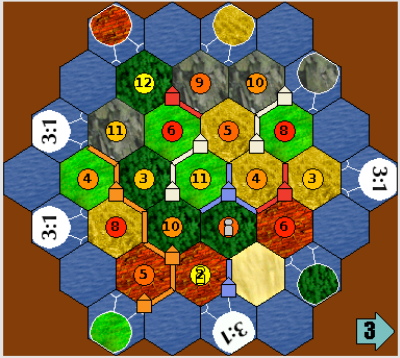
\includegraphics[width=80mm]{img/catan_board.png}
    \end{center}
    \caption{カタンの開拓者プレイ中ボードマップ~\cite{guhe2012trading}}
    \label{catan_board}
\end{figure}



\subsubsection*{資源の獲得}
各プレイヤーは順に、自分の手番が回ってくる。手番プレイヤーはまずサイコロを2つ振る。7以外の場合は、出た目の合計と同じ数字が書かれた地形から資源が産出することができる(出た目の合計が7だった場合は盗賊が出現するが、これについては後述)。サイコロの出目がでた数字の地形に接するように開拓地や街を建設していたプレイヤー全員が、開拓地1つ当たり1枚(街ならば2枚)の対応する資源カードを受け取ることができる。
自分の手番でなくても、サイコロの出目がでた地形に自分の開拓地が隣接していれば、資源を受け取ることができる。一方で、自分の手番であっても、サイコロの出目がでた地形に自分の開拓地が隣接していなければ、全く受け取ることはできない。

7が出た場合、手番のプレイヤーは他のプレイヤーから資源を1枚奪うことができる。資源を奪うプレイヤーを指定する必要があるため、他のプレイヤーは「どのプレイヤー」が「どのプレイヤー」から資源を奪ったかを知る事はできる。しかし、奪った資源は他のプレイヤーは知ることはできない。

\subsubsection*{発展方法}
得られた資源を用いて「建設」や「発展カード」を購入することができる。
自分のターンの間に、持っている資源で払える限り何回でも購入することができる。それぞれの建設コストは以下のようになっている。
\begin{itemize}
 \item 道路:「木」「土」を1つずつ
 \item 開拓地:「木」「土」「羊」「麦」を1つずつ
 \item 街:「麦」2つと「鉄」3つ
 \item 発展カード:「羊」「麦」「鉄」を1つずつ
\end{itemize}

を建設することができる。(建設方法に関しての詳細な方法はここでは述べない。)

発展カードには5種類あり、発展カードを購入する場合、山札からランダムに1枚獲得することができる。獲得した発展カードは、他のプレイヤーに見せる必要はない。発展カードは自分の手番にのみ使用でき、手番1回ごとに1枚までしか使用することはできない。

\subsubsection*{資源交換}
得られた資源を他の資源に変える方法は全部で3つ存在する。
\begin{itemize}
 \item 他のプレイヤーとの自由な資源交換
 \item 港を用いて条件にそった交換
 \item 同じ資源4つと、任意の資源1つを場から交換
\end{itemize}

上から順に交渉から得られる利益が多いとされているが、実際は状況や条件によって大きく左右されるため、自分の利益が最大となる交渉を見つける事が、勝利にいち早くつながる方法となる。

また、他プレイヤーと自由な資源交換を行なう場合、交渉内容として考えられる状態数は以下のの通りである。
プレイヤーAとプレイヤーBが交換するとする。
     プレイヤーAの手札の枚数$a$枚
     プレイヤーBの手札の枚数$b$枚 
とすると、交換する内容は最大で

\begin{eqnarray}
  F(a,b)=\sum_{i}\sum_{j}{}_a C _i\times{}_b C _j (0<i<a,0<j<b)
\end{eqnarray}

となる。(ただし、カードの種類の重複があると場合は減る。)$F(a,b)$通りの局面が考えられる。

\subsubsection*{勝利条件}
道路や建物を建設する事で、獲得したポイントの合計が最も早く10点に達したプレイヤーが勝利する。
得点源は以下のようなものがある。
\begin{itemize}
 \item 開拓地:1つ当り1点
 \item 街:1つ当り2点
 \item 得点カード:1枚当り1点(発展カードの25枚の中に5枚ある)
 \item 最も長い道路を作った(最長交易路ボーナス):2点
 \item 最も多く騎士カードを使った(最大騎士力ボーナス):2点(発展カードの中に14枚ある)
\end{itemize}

\subsubsection{カタンの特徴}

カタンには「マルチエージェント」「非決定的」「不完全情報」という大きく3つの特徴がある。
% この特徴をもつ理由をかんがえる上で、カタンの行動を大きく3つにわけるものとする。
% 「サイコロを振る」「戦略に基づいて建設を行う」「交渉を行う」

\subsubsection*{マルチエージェント}
カタンは一般的に4人で行われるゲームである。各々のプレイヤーは自ら考え自立的に行動し、複雑なアクションを行わなければならない。お互いのアクションはこのゲーム上内で影響を及ぼし合い、またこのゲーム上で完結している。
\subsubsection*{非決定的}
非決定的な状況は主に2つからおきる。
1つ目は「サイコロを振る」ときである。考えられる状況は11通りしかないが、それぞれの状況はランダムに起こりうるため、全ての状態について考える必要がある。また、それぞれの状態がおこる確率はバラバラであるため、確率の低いところでは探索回数を減らし、確率の高いところでは探索回数を増やすといったように、確率に応じた探索方法を提案する必要がある。
2つ目は「発展カード」を引くときである。発展カードは25枚の中からランダムに引かれるため、サイコロ同様考えられる状態数が爆発してしまう可能性がある。
\subsubsection*{不完全情報}
相手の情報とは大きく2つあり、「発展カード」と「手札」である。「交渉を行う」場合に不完全情報だと考えられる状態数が急激に増えてしまう。
それぞれ完全に知る事ができない理由は1つずつ存在する。
発展カードは、山札からランダムにカードが引かれ、引いたプレイヤーのみカードを知る事ができ他のプレイヤーは知る事ができない。
手札は、サイコロで7が出た場合に2人のプレイヤー間でカードの移動が行われ、移動したカードの種類は他のプレイヤーは知る事ができない。


% \subsection{JSettlers}

% JSettlersはカタンのAIで、GPL(General Public License)をもつオープンソースプロジェクトである。当初はAIの研究プロジェクトとして作成された~\cite{Jsettler}。
% Jettlersはカタンの一連の動作を行うことが可能である。JSettlersの戦術はある決まったルール(ルールベース)があり、エージェントはこれに基づいた行動を行う。JSettlersにおける交渉も、ルールベースで行われている。交渉を行う場合、相手プレイヤーの状況を認識し、計算ルールに乗っ取って勝率を計算する。勝率がある閾値を越えていない相手と交渉を行う。交渉内容は、自分の戦略に乗っ取って行われ、不足している資源を手に入れることを考え、相手が欲しい資源については考えない。そのため、お互いが満足する交渉が行われることは少ない。
% 本研究でJSettlersを交渉の相手に使用する場合は、まず、交渉を全く受けないプレイヤーと比較することで、JSettlersの交渉の有意性を示す必要がある。その後、交渉を受ける相手としてJsettlersを設定し、妥当な交渉を検討していく。

\subsection{SmartSettlers}
SmartSettlersは研究用に開発されたオープンソースのカタンAIである~\cite{SmartSettlers}。JSettlersをベースとして開発されており、単位時間あたりのシミュレーション回数を増やす目的で開発された。JSettlersはカタンのAIで、GPL(General Public License)をもつオープンソースプロジェクトである。当初はAIの研究プロジェクトとして作成された~\cite{Jsettler}。
SmartSettlersは交渉を除くカタンの一連の動作を行うことが可能である。SmartSettlersはランダムアクションとUCTアルゴリズムアクションの2つの戦術を有している。エージェントはこれに基づいた行動を行う。いずれもまずは、考えられる選択肢を全て列挙する。ランダムアクションはこれらのアクションの中からランダムに選択し行動する。UCTアルゴリズムアクションはアクションの中からUCTアルゴリズムに基づいて選択し行動する。
また、SmartSettlersは研究用に開発されたことから、自己対戦を行なう事が可能である。自己対戦は全てのプレイヤーがランダムにアクションを行なう場合、UCTアルゴリズムでアクションを行なう場合、いずれの場合も可能である。また、このとき「Intel(R) Xeon(R) CPU X5680 @ 3.33GHz」の実験環境のもとで、全てのUCTプレイヤーが1,000回プレイアウトを行なった場合、10数秒で1ゲームを終える事ができる。
さらに、カタンは席順によって勝率に差が出る事が一般的に知られている\cite{SmartSettlers}。SmartSettlerにおいて、全てのプレイヤーをランダムアクションとし、400ゲームの対戦実験を行なった結果、図4のような結果となった。

また、同様に1,000回シミュレーションを行なうUCTアルゴリズムプレイヤーにおいて400ゲーム行なった結果を以下の図5に示す。

\begin{figure}[t]
 \begin{minipage}{0.5\hsize}
    \begin{center}
      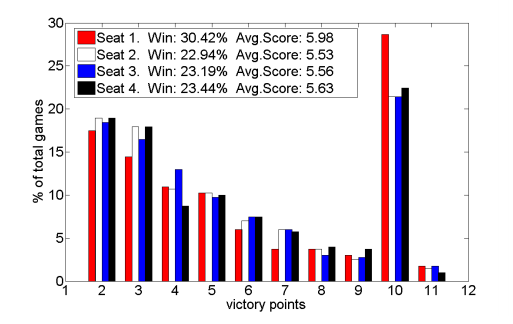
\includegraphics[width=80mm]{img/smart_random.png}
    \end{center}
    \caption{ランダムアクションによる席順の優劣\cite{SmartSettlers}}
    \label{smart_random}
 \end{minipage}
 \begin{minipage}{0.5\hsize}
    \begin{center}
      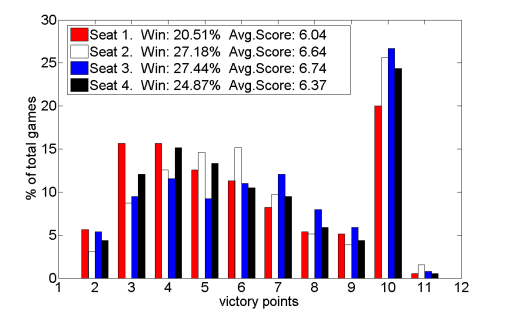
\includegraphics[width=80mm]{img/smart_uct.png}
    \end{center}
    \caption{UCTアクションによる席順の優劣\cite{SmartSettlers}}
    \label{smart_uct}
 \end{minipage}
\end{figure}

このように席順によって勝率が変わる原因として初期配置が考えられる\cite{SmartSettlers}。席順によって、勝率がかわることから、本研究で提案する手法を用いたアルゴリズムの結果は、席順を入れ替えて全ての席順に対して対戦実験を行い、勝率の平均値をとるものとする。


% 本研究でJSettlersを交渉の相手に使用する場合は、まず、交渉を全く受けないプレイヤーと比較することで、JSettlersの交渉の有意性を示す必要がある。その後、交渉を受ける相手としてJsettlersを設定し、妥当な交渉を検討していく。

\subsection{問題の簡単化}

カタンは「マルチエージェント」「非決定的」「不完全情報」なゲームである。本研究ではこの問題を簡単にするために、コンピュータは不完全情報ゲームよりも完全情報ゲームの方が先読みを得意としていることを利用して、以下のような方法で「マルチエージェント」「非決定的」「完全情報」なゲームであると考えることにする。理由は以下に示す。

実際のカタンでは相手の情報を完全に知る事はできない。そのため、カタンは不完全情報ゲームである。相手の情報とは大きく2つあり、「発展カード」と「手札」である。

発展カードを知る事はできないが、サイコロの出目と同様に相手の持つカードがどのような効果を発動するか非決定的であると考えればよい。

相手の手札を完全に知ることはできないが、相手の情報を完全に知っているものとして近似して考えることにする。これには大きく2つの理由がある。

1つは、サイコロで7が出る確率は1/6であり、カードの移動が行われる枚数は1枚だけである。これは使用されるカードの頻度と枚数に比べて十分小さい。
2つ目に、やりとりされたカードは多くの場合すぐに使用されるためである。
これらの理由から、多くの場合相手のカード情報が完全にわかっている状態であり、わからない状態であってもプレイにほとんど影響することはない。

よって、本研究では他のプレイヤーと交渉を行う上で、重要な要素である相手のカード情報は完全情報であると考える。すなわち、本研究で扱うカタンのAIは交渉を行うときに相手の手札カードを全て知っているものとする。

また、複数の相手と交渉を行なう場合、あるプレイヤーとの交渉条件をもとにして、別のプレイヤーに交渉を提示することが可能となる。これは2.4節で述べた通り、相手の戦略を知り、混合戦略を考える必要があるため非常に難しいとされる。
本研究では、全てのプレイヤーに対する交渉案の中から、自分の得られる利益の期待値が最大となる交渉を行なう。このとき、相手プレイヤー同士で交渉が行なわれる事はなく、また、自分が交渉できる回数は1回限りであるため、交渉するプレイヤーは1人だけになる。
そのため、プレイを行う環境はマルチエージェントであるが、交渉を行う上ではマルチエージェントシステムとして考えないものとする。

\subsection{交渉の方針}

本研究において交渉の利益計算方針は4つ存在する。また、交渉において提案と承諾について考える必要がある。
ただし、交渉は自分のターン1回につき1回のみ提案するできるものとする。また、交渉案は1対1交渉について考えるものとする。

\subsubsection*{受諾プレイヤー}
交渉を提案することはない。
交渉を受ける場合、相手が提示するすべての交渉案に対して、必ず受諾を選択する。

\subsubsection*{ランダムプレイヤー}
交渉を提案する場合、まず全てのプレイヤーに対して可能な交渉案を列挙する。但し、交渉を行なわないという選択肢もこの交渉案は含んでいるものとする。
これら交渉案の中から、均等な確率でランダムに交渉案を提案する。
交渉を受ける場合、半々の確率て受諾と拒否を選択する。

\subsubsection*{ルールベースプレイヤー}
交渉を提案する場合、まず全てのプレイヤーに対して可能な交渉案を列挙する。但し、交渉を行なわないという選択肢もこの交渉案は含んでいるものとする。
これらの交渉案の中から、一定のルールに基づき交渉前と交渉後の手札をポイント付けし交渉案の利益計算を行う。次に、提案手法である、「自己中心的交渉」「和交渉」「積交渉」「利益優先交渉」「交渉受諾優先交渉」のいずれかの評価関数のもと、最も良い評価値の交渉案を提案するものとする。本研究で用いるルールは以下のように設定するものとする。

\begin{itemize}
 \item 道が引ける場合 3ポイント
 \item 家が建てられる場合 10ポイント
 \item 街が建てられる場合 15ポイント
 \item 自分と交渉相手の点差 例)自分が5点と相手が7点の場合、-2ポイント
\end{itemize}

お互いがwin-winな交渉をもちかけることを前提にすると、同ポイントの場合、自分より点数の高いプレイヤーよりも自分よりも点数の低いプレイヤーに交渉を持ちかける方が勝率があがると予想される。
交渉を受ける場合、上記のルールに基づき評価関数を用いて得た評価値がプラスになる交渉案であれば必ず受諾し、0、もしくは評価値がマイナスの場合は拒否するものとする。
\subsubsection*{UCTプレイヤー}
交渉を提案する場合、まず全てのプレイヤーに対して、可能な交渉案を列挙する。但し、交渉を行なわないという選択肢もこの交渉案は含んでいるものとする。これら各々の交渉案に対して、N回のプレイアウトを行い各プレイヤーの勝率を計算し、これをもとにして利益計算を行なう。次に、提案手法である、「自己中心的交渉」「和交渉」「積交渉」「利益優先交渉」「交渉受諾優先交渉」のいずれかの評価関数のもと、最も良い評価値の交渉案を提案するものとする。
交渉を受ける場合、交渉を受ける前と受けた後においてN回プレイアウトを行い、勝率を計算する。この勝率をもとに、評価関数を用いて得た評価値がプラスになる交渉案であれば必ず受諾し、0、もしくは評価値がマイナスの場合は拒否するものとする。

\section{評価}
\subsection{交渉を行なわない場合の比較}
交渉を行なう前に、カタンの開拓者を知能的にプレイしない限りは交渉を行なうことすら不可能である。本研究の実験環境であるカタンの開拓者をプレイする実験を行った。
まず、全くUCTアルゴリズムによる探索を行なわないプレイヤー同士での実験結果を図6に示した。このプレイヤーはUCTアルゴリズムを用いていないため、自分のターンで考えられる行動のリストからランダムに選択をおこない行動する(以下、交渉なしランダムプレイヤー)。下記実験では1,000回の対戦実験を行いその結果を示す。本実験環境では、1ゲームあたり2~3秒程度で終えることができる。
\begin{figure}[b]
    \begin{center}
      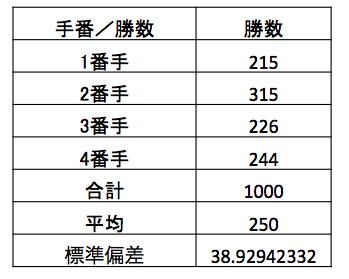
\includegraphics[width=50mm]{img/arrangement.png}
    \end{center}
    \caption{席順と勝数の比較}
    \label{arrangement}
\end{figure}

結果より、関連研究であった通り\cite{SmartSettlers}席順による優劣があることが確認された。以降、プレイヤーのアルゴリズムを変更した場合は全ての席順において対戦実験を行い、その平均値の勝率を考えるものとする。 
次にUCTアルゴリズムをカタンの開拓者に適用した結果を図7に示す。UCTアルゴリズムを用いたプレイヤー(以下、交渉なしUCTプレイヤー)は次の自分の行動をUCTアルゴリズムを用いて選択し行動する。交渉を行なわないため、交渉に関する行動はこの選択肢には入らないものとする。下記の図の実験では「3人の交渉なしランダムプレイヤーと1人の交渉なしUCTプレイヤー」を用いて実験を行なった。UCTアルゴリズムのプレイアウトの回数を変更する実験を行なった。プレイアウトの回数が多いプレイヤーの方が、プレイアウトの回数が少ないプレイヤーに比べて、より良い行動を選択できると予想される。よって、プレイアウト回数の多いプレイヤーの方がランダムプレイヤーに対して、より良い勝率をおさめる事ができると予想される。下記実験では、席順によって勝率が変化する事から、各々の席順に対して交渉なしUCTプレイヤーを配置し、「1人の交渉なしUCTプレイヤーと3人のランダムプレイヤー」として1,000回の対戦実験を行った。その勝率を示す。

\begin{figure}[b]
    \begin{center}
      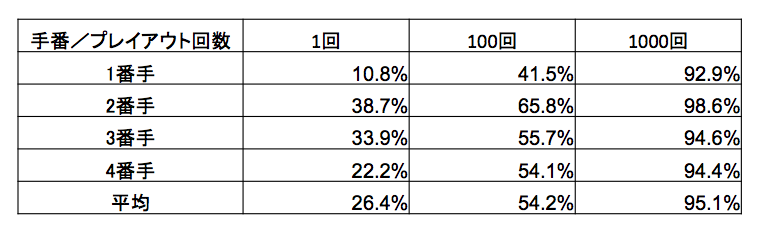
\includegraphics[width=120mm]{img/playout.png}
    \end{center}
    \caption{プレイアウト回数による勝率の変化}
    \label{playout}
\end{figure}

表より、プレイアウトの回数が順に、1回の場合はUCTプレイヤーに対して26.42\%、100回の場合はUCTプレイヤーに対して54.2\%、1,000回の場合はUCTプレイヤーに対して95.1\%の勝率を得た。勝率は各席順の平均値を用いるものとする。4人プレイを行なっているため、勝率が25\%以上であればよい。プレイアウトの回数が1回の場合はランダムに行動を選択する場合とかわらないため、有意な実力差は得られなかった。しかしながら、プレイアウトの回数を100回、1,000回にした場合、交渉なしランダムプレイヤーは54.2\%、95.1\%と優位な結果を得る事ができた。このことから、カタンにおけるUCTアルゴリズムは有効であることがわかる。よって、交渉においても、UCTアルゴリズムが有効であると期待される。
また、本研究で交渉を扱う場合、交渉なしUCTアルゴリズムでランダムプレイヤーに対して最も良い結果を残した、1,000回のプレイアウト回数を用いたカタンAIを用いて、実験を行なうものとする。


\subsection{交渉の利益計算方法の比較}
交渉の利益計算を行なう方法として受諾プレイヤー、ランダムプレイヤー、ルールベースプレイヤー、UCTプレイヤーを用意した。下記の図8はその対戦実験の結果である。
現実世界の交渉において、違う種類の資源を使用し、異なる分量で提示する交渉が存在する。カタンにおける交渉でも異なる分量で行なわれる交渉が存在する。例えば、自分は2枚資源を提示し、相手は資源を3枚提示するといった多対多の交渉が許されている。交渉内容はカード枚数(分量)による影響を受ける可能性がある。1対1交渉の利益計算で最もよい成果を出したルールベースプレイヤーを用いて「3人の受諾プレイヤーと1人のルールベースプレイヤー」の実験を行なった。枚数による影響を考えるため、最も単純な2対1交渉を考えるものする。提示する側のプレイヤーは必ず同種または異種のカードが合計2枚になるように提示し、受ける側のプレイヤーは1種提案するものとする。ルールベースプレイヤーは自分の利益が最大となる交渉案を提示するものとする。ルールベースプレイヤーが自分にとって有利な提案ができている場合は、25\%以上の勝率が期待される。また実験結果より、席順が影響することから全ての席順において1,000回対戦実験を行い、得られた勝率の平均値を最終的な勝率にしている。
結果をの図8に示す。

\begin{figure}[b]
    \begin{center}
      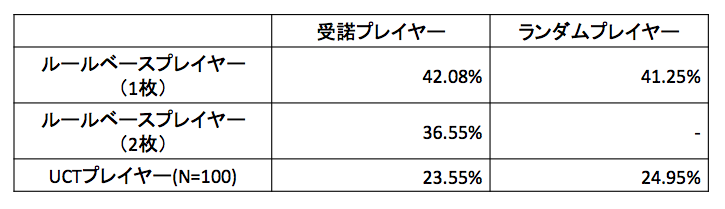
\includegraphics[width=120mm]{img/eachplayer.png}
    \end{center}
    \caption{各プレイヤー同士の対戦実験結果}
    \label{eachplayer}
\end{figure}


図より、1対1の交渉では勝率が42.08\%だったのに対し、2対1交渉では勝率が36.55\%といずれの場合も有利な交渉を提案できている。しかし、枚数を増やすことによって、勝率が下がっていることが分かる。よって、まずはUCTプレイヤーとルールベースプレイヤーが有利な提案ができているかを検証するために、1対1の交渉において実験するものとする。
本研究では「3人の受諾プレイヤーと1人のルールベースプレイヤー」と「3人の受諾プレイヤーと1人のUCTプレイヤー」との対戦実験の行なった。前述の通り、交渉を行なう枚数は1対1交換のみにしている。UCTプレイヤーの各交渉案に対するプレイアウト回数は100回とした。また、ルールベースプレイヤー、UCTプレイヤー共に自分の利益が最大となる交渉案を提示するものとする。
また同様にして、「3人のランダムプレイヤーと1人のルールベースプレイヤー」と「3人のランダムプレイヤーと1人のUCTプレイヤー」としてランダムプレイヤーとの対戦実験も行なった。
ランダムプレイヤーは有利な交渉を提示する上でのベースラインとして考えるものとする。
結果より、ルールベースプレイヤーが全受諾プレイヤーに対して42.08\%(前述と同じ)と有意な実力差を残していることから、自分にとって有利となる利益計算を行い、交渉案を提示していることが分かる。一方で、UCTプレイヤーは受諾プレイヤーに対して23.55\%と25\%より低い勝率となった。すなわち、自分にとって有利な利益計算を行なうことができず、結果として有利な交渉案を提示できなかったと考えられる。
また、ランダムプレイヤーに対してもルールベースプレイヤーは41.25\%と高い勝率をおさめたが、UCTプレイヤーはランダムプレイヤーに対しても24.95\%と有意な実力差を得る事はできなかった。
UCTプレイヤーが良い結果を残せなかった原因を考えていく。ルールベースプレイヤーはUCTプレイヤーに比べて、ランダムプレイヤーと受諾プレイヤーに対し、良い勝率をおさめていることから、ルールベースプレイヤーはUCTプレイヤーよりも良い交渉案を提示していると考えられる。よって、ルールベースプレイヤーの交渉案は正しいと仮定のもと、考えていくものとする。また、UCTアルゴリズムはプレイアウトの回数によって精度を向上できることから、プレイアウトの回数を各交渉案において、100回の場合と1,000回の場合を比べるものとする。UCTプレイヤーとルールベースプレイヤーとの交渉案の一致率を以下に図9,10に示す。それぞれ、338,758回、105,868回の交渉を行なった。

\begin{figure}[htbp]
 \begin{minipage}{0.5\hsize}
    \begin{center}
      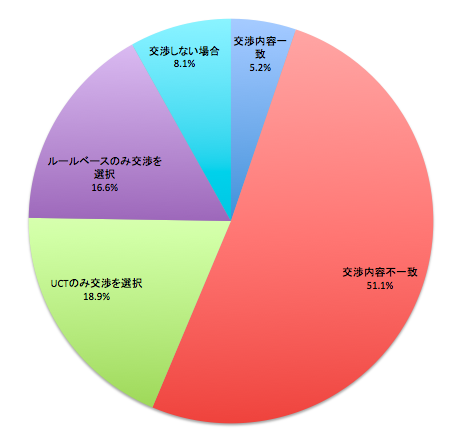
\includegraphics[width=70mm]{img/match_100.png}
    \end{center}
    \caption{UCT(N=100)とルールベースの交渉案選択の一致率}
    \label{match_100}
 \end{minipage}
 \begin{minipage}{0.5\hsize}
    \begin{center}
      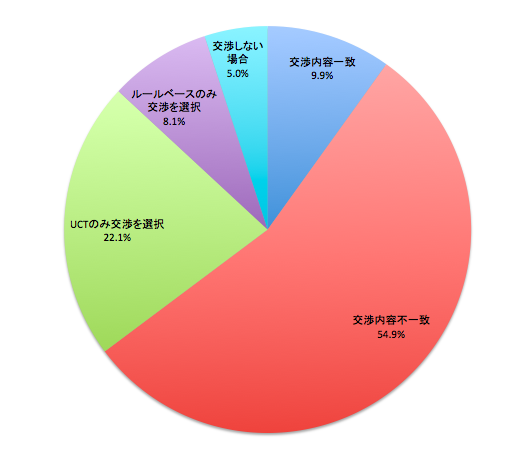
\includegraphics[width=80mm]{img/match_1000.png}
    \end{center}
    \caption{UCT(N=1000)とルールベースの交渉案選択の一致率}
    \label{match_1000}
 \end{minipage}
\end{figure}

ルールベースプレイヤーとUCTプレイヤーの交渉案の全体の一致率(交渉を行なわない場合の一致率と、交渉を行なう場合の一致率を合わせた割合)を考える。
プレイアウトの回数が100回の場合の交渉案の一致率は、ルールベースプレイヤーとUCTプレイヤー共に交渉を行ない同じ交渉案を選択する場合(5.2\%)と交渉を行なわない場合(8.2\%)を合わせた13.4\%であった。また、
プレイアウトの回数が1,000回の場合の交渉案の一致率は、ルールベースプレイヤーとUCTプレイヤー共に交渉を行ない同じ交渉案を選択する場合(9.9\%)と交渉を行なわない場合(5.0\%)を合わせた14.4\%であった。ランダムプレイヤーとルールベースプレイヤーの交渉案の一致率は、6.1\%なので、ランダムよりは良い精度で交渉案を選択できているものの、十分でないと考えられる。
しかしながら、ルールベースプレイヤーとUCTプレイヤー共に交渉を行なう場合において、プレイアウトの回数を100回のUCTプレイヤーはルールベースプレイヤーと10.2\%の一致率であるのに対して、プレイアウトの回数が1,000回のUCTプレイヤーは18.1\%と大きく向上した。このことから、プレイアウトの回数を増やすことで、良い交渉案を選択できると考えられる。また、本研究で受諾プレイヤーに対して良い結果をおさめられなかった原因として、プレイアウトの回数が十分でなかったと考えられる。しかしながら、100回のプレイアウトで1ゲーム当たり700秒程度必要であり、1,000回プレイアウトを行なった場合、1ゲーム当たり6,600秒程度の時間が必要となる。プレイアウトの回数を増やす事によって線形にプレイ時間が増えてしまうことは大きな課題である。一部の有力でない交渉案をルールベース等で除いてから、探索を行なうといった工夫が必要となる。

また、UCTプレイヤーは序盤では良い交渉案を提案するものの、終盤になるとよい交渉案を選べなくなることがあった。図11はUCTプレイヤーとルールベースプレイヤーの交渉案の一致率を縦軸:一致率、横軸:勝率として表したものである。横軸の勝率とは、UCTアルゴリズムでシミュレーションを行なった結果、選択された交渉案において、最も勝率が高かったプレイヤーの勝率を示している。ただし、自分が最も勝率が高かった場合は考えないものとする。

\begin{figure}[b]
    \begin{center}
      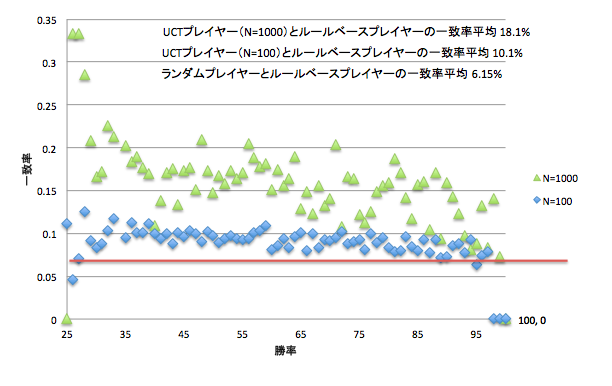
\includegraphics[width=120mm]{img/match_100_1000.png}
    \end{center}
    \caption{UCTプレイヤーとルールベースプレイヤーの交渉選択の一致率(N=100,N=1000)}
    \label{alignment}
\end{figure}

図より、前述の通りプレイアウト回数が1,000回の方が100回よりも高い一致率となっている。また、いずれもルールベースよりも高い一致率になっていることがわかる。
また図より、勝率が高くなるほど、一致率が下がっていく傾向にある。プレイアウト回数が1,000回の場合では、相手プレイヤーの勝率が35\%以下の時に平均よりも高い一致率を示しているにも関わらず、勝率が90\%以上になると、プレイアウト回数が100回の一致率やランダムプレイヤーに近い一致率になってしまう。これは勝率が拮抗している序盤では良い交渉案を提示しているものの、勝率に差がついてくる終盤になると良い交渉案を選べない原因だと考えられる。相手の勝率が高くなってしまうと、良い交渉を提案できなくなる理由として、自分の勝率計算の精度が悪くなることが考えられる。全ての交渉案に対して1,000回のプレイアウトを行なうが、いずれの交渉案においても一度の交渉で大きく勝率が変わる事はないため、相手の勝率は90\%付近となっている。そのため、残りの10\%である100回のプレイアウト回数の中から良い交渉案を見つける必要があるが、プレイアウト回数を増やしたにも関わらず、良い一致率を得ることができなくなってしまう。よって、勝率計算において相手の勝率が高くなった場合には一定の重みをつけて計算することで、精度の悪化を防ぐ事が考えられ、今後の課題である。

以上より、UCTプレイヤーの勝率が受諾プレイヤー、ランダムプレイヤーに対して良い結果を残せなかった原因として、「プレイアウト回数が不十分であったこと」「相手の勝率が高くなった場合での精度悪化」が考えられるため、これらの改善を行なうことが課題となる。また、UCTプレイヤーよりもルールベースプレイヤーの方が良い結果を残した事から、ルールベースプレイヤーのほうが良い利益計算を行なっていると考え、交渉の評価選択手法を提案する上で、ルールベースプレイヤーを用いる事にする。


\subsection{交渉の評価基準の比較}
本研究の提案手法として、良い交渉案を選ぶ評価関数に、以下の5つを示した。自分の利益のみしか考えない「自己中心的交渉」を行なうプレイヤーをベースラインとして扱い、次に、交渉の成功率よりも相手の利益を優先にした「利益優先交渉」と交渉の成功率を優先した「受諾優先交渉」がある。また、お互いの利益をバランスよく配分することで自分の利益と交渉の成功率をバランスよく配分する手法として「和交渉」「積交渉」を提示した。交渉の評価基準を比較する上で、交渉の方針の中で最も良い利益計算を行なっているルールベースプレイヤーを用いることにする。まず、提案を行なうときに、同じ利益計算関数のもと、異なる評価関数を用いて評価実験を行なった。「1人の利益優先交渉プレイヤーと3人の自己中心的交渉プレイヤー」、「1人の受諾優先交渉プレイヤーと3人の自己中心的交渉プレイヤー」、「1人の和交渉プレイヤーと3人の自己中心的交渉プレイヤー」、「1人の積交渉プレイヤーと3人の自己中心的交渉プレイヤー」について対戦実験を行なった。ただし、全てのプレイヤーにおいて受諾するときの評価関数は同一のものとし、その評価関数は「自分の利益が0よりも高くなる交渉は全て受諾する」としている。実験結果を図12に示す。

\begin{figure}[b]
    \begin{center}
      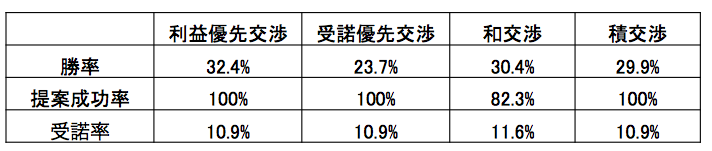
\includegraphics[width=120mm]{img/baseline.png}
    \end{center}
    \caption{ルールベースの評価値を用いた対戦実験結果}
    \label{rulebase_value}
\end{figure}


受諾時に同じ利益関数を使っており、少しでも利益がある場合は受諾するため、自分の評価関数のもとで相手がプラスになる交渉案を提示する、利益優先交渉、受諾優先交渉、積交渉では必ず100\%の受諾率となった。和交渉で100\%とならなかったのは、相手の利益がマイナスではあるが自分の利益と相手の利益の合計で最も高くなる交渉案を提示する場合があったからだと考えられる。
必ず相手が受諾するため、自分にとって最も利益の高い交渉案を常に提案できる利益優先交渉が32.4\%と最も高い勝率となった。しかし、受諾優先交渉では自分にとって小さな利益しか得られないにも関わらず相手に大きな利益を与えてしまうため、自己中心的プレイヤーのもとで25\%以上の勝率とはならなかった。また、バランス型の評価関数である積交渉が自己中心的交渉プレイヤーに対して29.88\%と高い勝率をおさめたことから、自分の利益を一定数確保した交渉案を提示する必要があると考えられる。
実際の交渉では、交渉に楽観的で自分の評価では相手にとって利益がない時でも相手プレイヤーが交渉を受諾する場合があり、また一方で、交渉に関して悲観的なプレイヤーでは、相手にとって利益があると自分が考えていた場合でも、受諾しない場合がある。そこで、これらの評価関数が、交渉に対して楽観的な環境と悲観的な環境でも同様の成果が得られるかどうかの評価実験を行なった。交渉を提案するときには、4つの評価手法を用いてそれぞれ3人の自己中心的プレイヤーとの対戦実験を行なった。全てのプレイヤーにおいて受諾するときの評価関数は同一のものとし、その評価関数は楽観的な環境下では「交渉をしない場合の評価値に比べて-10\%の交渉案も受諾してしまう」ものとし、また一方で、交渉に関して悲観的なプレイヤーのもとでは、「交渉をしない場合の評価値に比べて+10\%の交渉案ならば受諾しない」
ものとした。結果を以下の図13、14に示す。   

\begin{figure}[b]
    \begin{center}
      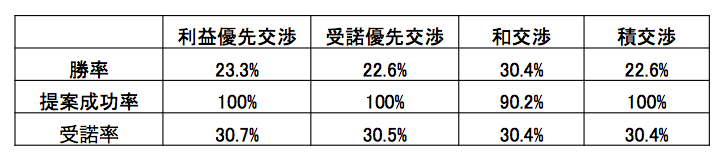
\includegraphics[width=120mm]{img/nego_positive.png}
    \end{center}
    \caption{交渉に楽観的な環境下での対戦実験結果}
    \label{envirn_positive}
\end{figure}

\begin{figure}[b]
    \begin{center}
      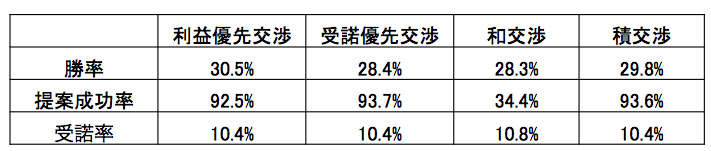
\includegraphics[width=120mm]{img/nego_negative.png}
    \end{center}
    \caption{交渉に悲観的な環境下での対戦実験結果}
    \label{envirn_negative}
\end{figure}



交渉に関して楽観的な環境においては、和交渉のみが30.4\%と25\%を超える勝率となった。その他の評価関数が自己中心的な評価関数に比べて悪い結果になった原因として、交渉案の受諾
に失敗したと考えられる。全てのプレイヤーが楽観的な交渉をおこなった結果、自己中心的なプレイヤーの交渉案を受諾する率が30\%程度と楽観的
でない場合の11\%に比べて大きく上昇した。そのため、自分にとって不利な交渉案を多く受諾してしまう結果となった。和交渉が楽観的な環境下でも高い勝率を残したのは、相手から悪い交渉を行なう中で、自分も相手にとって悪い交渉案を提案していたからだと考えられる。
また、交渉に関して悲観的な環境下では、自己中心的交渉に対して全ての評価関数が25\%以上の結果を残した。否定的な環境下では、自分にとって不利な交渉案を提示される可能性のある自己中心的な交渉案は受諾されにくいと考えられる。実験結果より、悲観的な環境下では、自己中心的交渉は10\%と悲観的でない場合の11\%に比べてわずかではあるが受諾率が下がっていることがわかる。
悲観的な環境下では自己中心的な交渉を誤って受諾することがなくなる一方で、自分の交渉案も受諾されにくくなる。そのため、いずれの評価関数でも悲観的でない環境下に比べて相手の受諾率は下がってしまった。利益優先交渉(30.5\%)、和交渉(28.3\%)では、この影響により悲観的でない場合に比べて勝率が下がってしまったと考えられる。

以上より、交渉を受諾する時、自分では良い交渉案だと思っている交渉案に対して、結果悪い交渉案であった場合があるため、悪い交渉案を受けないよう受諾基準をあげた評価関数が良い結果を残すと考えられる。また、提案する時、実際の交渉では相手の受諾評価基準が自分の評価基準よりもずれていて、楽観的か悲観的かわからないため自己中心的な交渉案を提示するだけでは、高い勝率を残すことはできない。また、評価基準が自分よりもずれていることを利用して、悪い交渉案を混ぜることで勝率を高めることができると考えられる。

これらの実験では受諾するときには、提案するときと同じ評価関数を用いてきた。実際の交渉においては、交渉を行なうプレイヤーは異なる利益計算関数を用いて利益計算を行い、計算された利益を用いて自分の評価関数によって提案、受諾を行なう。お互いの利益計算関数と評価関数が異なっていることにより、相手にとって利益がプラスであるから必ず受諾されると予想し提案した交渉案でも、受諾されないことがある。そのため、同じ評価関数を用いた前述の実験のように提案成功率が100\%になることはないと考えられる。よって、異なる利益計算関数と異なる評価関数を用いた実験を行なう必要がある。
本研究では、楽観的な利益計算を行ない、自己中心的な評価関数を用いて交渉案を選択、受諾を行なう「楽観的自己中心交渉プレイヤー」と、悲観的な利益計算を行ない、自己中心的な評価関数を用いて交渉案を選択、受諾を行なう「悲観的自己中心交渉プレイヤー」を用いて、提案手法である4つ評価関数の性能評価を行なった。楽観的自己中心交渉プレイヤー、悲観的自己中心交渉プレイヤーは、受諾するとき自分の利益計算関数を用いて得た利益が交渉を行なう前に比べてプラスになる場合は必ず受諾するものとする。また、楽観的な利益計算関数は、交渉を行なう場合の評価値をルールベースの評価値よりも10\%多く見積もってしまう関数とし、悲観的な利益計算関数は、交渉を行なう場合の評価値をルールベースの評価値よりも10\%少なく見積もる関数とする。
また、「利益優先交渉」「受諾優先交渉」「和交渉」「積交渉」の利益計算関数はルールベースの評価値を用いるものとし、この利益計算関数によって得た利益により、評価関数を用いて提案、受諾を行なう。評価関数によって得た最終的な交渉の期待値がプラスの場合にのみ受諾を行なうものとする。
結果を以下の表に示す。

\begin{figure}[t]
    \begin{center}
      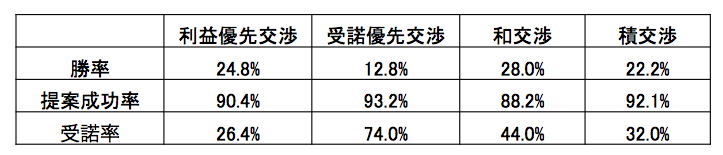
\includegraphics[width=120mm]{img/eva_positive.png}
    \end{center}
    \caption{各々の評価関数を用いた楽観的な自己中心プレイヤーに対する対戦実験結果}
    \label{player_positive}
\end{figure}


\begin{figure}[t]
    \begin{center}
      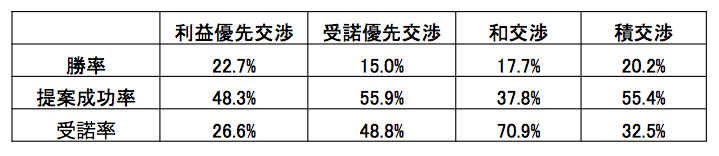
\includegraphics[width=120mm]{img/eva_negative.png}
    \end{center}
    \caption{各々の評価関数を用いた悲観的な自己中心プレイヤーに対する対戦実験結果}
    \label{player_negative}
\end{figure}

実験結果より、提案成功率と受諾率について考えるものとする。楽観的な交渉プレイヤーに対してはいずれの評価関数も90\%前後と高い提案成功率を残した。受諾プレイヤーが12.8\%と楽観的環境下の22.6\%に比べて大きく勝率が減少してしまった理由として、提案の受諾率があがったことが考えられる。他の評価関数に比べて、74.0\%と高い受諾率になっている。受諾優先交渉では、自分にとって利益が少なくても、相手の利益が大きい交渉案を受け入れてしまうため、受諾率は高かったものの、勝率に結びつくことはなかった。また、悲観的なプレイヤーに対して和交渉では他の実験に比べて17.7\%と低い勝率となった。この結果においても、自分の提案成功率が37.8\%であるのに対し、受諾率が70.9\%と高い受諾率となっている。和交渉の評価関数では、相手の利益と自分の利益の和が交渉を行なう前と後でプラスになっている、かつ、自分にとって利益のある交渉案を受け入れている。そのため、楽観的なプレイヤーに対する受諾プレイヤー同様、相手にとって大きな利益はあるが、自分にとって利益の少ない交渉案を悲観的な交渉プレイヤーに多く提示されたものだと考えられる。大きく受諾率があがったのは、悲観的プレイヤーの利益関数によるものだと考えられる。また、相手に対する提案成功率が37.8\%と楽観的プレイヤーに対して88.2\%だったのに対して大きく減少した。これは、和交渉だけではなく、楽観的プレイヤーに対して90\%前後の提案成功率を残していた他のプレイヤーにおいても同様のことがいえる。楽観的な交渉プレイヤーに比べて悲観的交渉プレイヤーでは全体の勝率が下がったのは、提案成功率が下がったことが原因だと考えられる。
以上より、良い交渉を行なう評価関数は、「提案成功率を高める」「受諾率を下げる」評価関数である必要がある。また、敵プレイヤーであった、自己中心的交渉プレイヤーが受諾率は高く提案成功率は低い中で他のプレイヤーに対して高い勝率を残したことから、交渉成功率を考えない純粋な「自分にとっての利益」と「相手に与える損益」の要素が関係していると考えられる。
このことから、全ての実験において得られた結果から、交渉の成功率と受諾率の関係の比と勝率の関係を表した図を以下に示す。



\begin{figure}[t]
    \begin{center}
      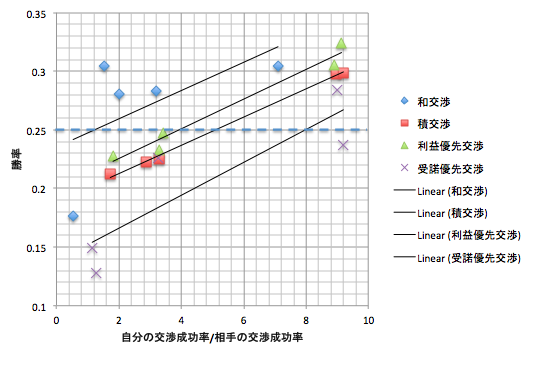
\includegraphics[width=120mm]{img/relation_winrate.png}
    \end{center}
    \caption{評価関数の勝率と交渉成功率}
    \label{win_rate}
\end{figure}




図より、全ての評価関数において(自分の交渉成功率/相手の交渉率)の割合が高まれば高まるほど良い勝率を残すことができると考えられる。このことからも、交渉における「提案成功率」と「受諾率」が関係していると考えられる。また、和交渉ではばらついたものの、利益優先交渉や、積交渉のように近似直線を描くと一定の直線上にのっていることがわかる。また、図よりこれら4つの直線の傾きは一定であるが、評価関数によってその近似直線が上下することがわかる。評価関数によって近似直線が上下する原因として、「自分にとっての利益」と「相手に与える損益」のバランスによるものと考えられる。バランス型の交渉である和交渉では、相手に与える損益を加えたことが高い勝率に結びついたと考えられる。また、受諾優先交渉、利益優先交渉と積交渉では相手に与える損益がないため、自分の得られる利益が大きい順に高い結果を残すことができたと考えられる。利益優先や受諾優先ではなくバランスよく利益配分を行なう和交渉がもっともよい結果を残したことから、「自分にとっての利益」と「相手に与える損益」をバランスよく配分する評価関数が最もよい評価関数だと考えられる。

また、相手プレイヤーによって受諾率や提案成功率が変化することから交渉において相手の評価関数に大きく影響をうけるものと考えられる。相手が楽観的な交渉プレイヤーであれば、相手に与える損益が多い評価関数は、良い結果を残せるが、悲観的な交渉プレイヤーでは悪い結果となってしまう。先行研究~\cite{ito2012complex}においても、周りの環境によって結果が大きく左右されていた。

以上の実験結果より、交渉において「提案成功率」「受諾率」「自分の利益」「相手の損益」を考えることが必要であることを明らかにした。提案成功率と受諾率は相手プレイヤーの評価関数に依存する。また、「相手の損益」を考慮するのは、自分では悪い交渉案だと思っている交渉案においても、相手との評価基準が自分よりもずれていることを利用して、悪い交渉案を混ぜることで勝率を高めることができると考えられるためである。

\section{おわりに}
\subsection{まとめ}
本論文では、交渉の利益計算手法をルールベースとUCTアルゴリズムの2つを提案し、UCTアルゴリズムの交渉への適用を試みた。また、交渉の評価関数を5つ提案し、対戦実験を行なう事で、交渉における4つの要素を明らかにした。
UCTアルゴリズムによる利益計算はプレイアウトによる勝率のフィードバックを用いることにより行なった。受諾プレイヤーに対して有意に高い勝率を残したルールベースプレイヤーと交渉案の一致率を確認することにより、UCTアルゴリズムによる利益計算の問題点を明らかにした。
また、交渉の評価関数の実験では、利益を優先する評価関数と交渉の成功率を高める評価関数とこれらをバランスよく配分した評価関数を用意し、自己中心的なプレイヤーに対して様々な環境において検証を行なった。
交渉においては、自分の利益計算関数と評価関数が相手の利益計算関数と評価関数にずれが生じていることから、自分では悪い交渉案だと思っている交渉案においても、相手との評価基準では、良い交渉案だと判断する場合があるため、悪い交渉案を混ぜることが有効であった。このことから、「提案成功率」「受諾率」「自分の利益」のみならず、「相手の損益」を考慮した評価関数を生成する必要があると考えられる。



\subsection{今後の課題}
交渉を行なうに上で

\begin{itemize}
 \item 全てのプレイヤーに対して可能な交渉案のリストアップ
 \item 各交渉案の利益の見積もり
 \item 評価関数による各交渉案の期待値計算
 \item 交渉案の提示
\end{itemize}
の順番で行なわれる。
本研究では可能な交渉案をリストアップするときに、問題を簡単化するために、1対1交渉に限定した。現実世界での交渉では、提示する交渉案は資源の種類のみならず、交渉の量が異なる交渉案が提示される。よって、多対多の交渉モデルを構築する必要がある。
また、本研究では各交渉案の利益計算を行なうためにUCTアルゴリズムを適用することを試みた。UCTアルゴリズムにおいて良い結果を残せなかった原因として、シミュレーション回数と負けているときに自分にとって有利な交渉案を提示できなかった。シミュレーション回数は指数的に増加してしまうことから、最後までプレイアウトを行なわず、一定の時間でシミュレーションを打ち切り、新しく評価関数を用意して盤面を評価し、その時点で評価値が最も高いプレイヤーを暫定の勝利者とするといった工夫が必要となる。また、負けているときにはシミュレーション回数を増やす事で精度を高められなかったことから、重み付けを行なうことによって精度を保つ必要があり、パラメータを調整することで、この重み付けの方法を調査する必要がある。
また、本研究では交渉案を提示する回数を1回とし、1回で自分の利益を最大にする評価値を返す評価関数を提案した。しかし、実際の交渉では、何回か交渉を行なう事でお互いの妥協点を探っていく事になる。さらに、妥協点を探すときには、先行研究にあるとおり、悪い交渉案を先に提示しておいて誤った認識を相手に与える事で有利な交渉を行なうといった方法が考えられる。また、時間や交渉回数が限られてくる場合には、交渉を行なう手順が複雑となる。


% 交渉を行うために、評価値を生成するUCTアルゴリズムの実装をJSettlersを動作させる環境を整備した。また、JSettlers上で動くUCTアルゴリズムの実装を現在行っている。実装を終えた後、評価値を用いて交渉を行う評価関数の生成に入る。
% \subsection{今後の計画}

% 今後の課題として
% \begin{itemize}
%  \item 対戦実験による評価値の調査
%  \item 評価値に基づく評価関数の調査
%  \item 現実世界の交渉における効果の調査
% \end{itemize}

% があげられている。これらの課題に取り組くむために、今後は以下の研究を進める必要がある。

% \begin{itemize}
%  \item 様々な局面を用意し対戦実験を行い、UCTを計算する評価値を調査する
%  \item 評価値に基づく交渉の評価関数を用意して、再度様々な局面に対する対戦実験を行い交渉の評価関数を調査する
% \end{itemize}

\newpage
\addcontentsline{toc}{section}{謝辞}
\section*{謝辞}

本研究を進めるにあたって、多くの方にお世話になりました。
指導教員である近山隆教授には研究の方向性に始まり、様々な面でアドバイスをいただきました。また、研究に対する心構えを教えてくださいました。
同じく、指導教員である鶴岡慶雅准教授には、研究の内容や進め方について数多くのアドバイスをいただきました。
マンチェスター大学の三輪誠さんには、技術的なアドバイスや論文紹介など細部にわたって助けていたただきました。
研究室博士の浦晃さんには、本研究で行なうべき実験の方向性に関してアドバイスをいただきました。  
研究室の皆様には、研究生活のみならず、技術的な面でも大変お世話になりました。多大な支援をいただきありがとうございました。
この場を借りて厚くお礼申し上げます。

\newpage
\addcontentsline{toc}{section}{参考文献}

\bibliographystyle{junsrt}
\bibliography{final_ver0}



\end{document}
